\section{Manajemen Memori}
\par
Kinerja komputer sangat dipengaruhi oleh Organisasi dan manajemen memori.
Manajemen memori melakukan tugas yang penting dan sangat komplek berkaitan dengan :
\begin{enumerate}
\item Memori utama sebagai sumber daya yang harus dialokasikan dan dipakai bersama antar sejumlah proses yang aktif
\item Upaya agar pemrogram atau proses tidak dibatsi kapasitas memori fisik di sistem komputer.
\end{enumerate}

Fungsi Manajemen memori 
\begin{enumerate}
\item mengelola informasi memori yang dipakai dan tidak dipakai
\item mengalokasikan memori ke proses yang memerlukan
\item Mendealokasikan memori dari proses telah selesai.
\item Memgelola swapping antar memori utama dan disk
\end{enumerate}

\section{Jenis Memori}
\subsection{Jenis Memori Yang Populer}

Berikut ini beberapa jenis memori yang banyak digunakan pada saat ini sebagai berikut:

\begin{enumerate}

\item RAM (Random Acces Memory) adalah memory sebagai tempat penyimpanan sementara pada saat komputer di jalankan dan dapat di akses secara acak atau random. Fungsi dari RAM adalah mempercepat pemrosesan data pada komputer. Semakin tinggi jumlah RAM yang Anda miliki, semakin cepat pula kemampuan komputer Anda dalam mengeksekusi.
Jenis Memory RAM :

\begin{itemize}

\item EDORAM (Extended Data Out RAM)  
\item SDRAM (Synchronous Dynamic RAM)  
\item DDR SDRAM (Double Data Rate Synchronous Dynamic RAM) 
\item RDRAM (Rambus Dynamic RAM)

\end{itemize}	

\item Menurut artikel yang berjudul Evolusi Komputer, Kinerja Komputer Dan Interconnection Networks Dalam Perkembangan Dunia Teknologi Informatika menyebutkan bahwa Registers adalah media penyimpan internal CPU yang digunakan saat proses pengolahan data. Memori ini bersifat sementara, biasanya hanya digunakan untuk menyimpan data saat diolah ataupun data untuk pengolahan selanjutnya. Sistem dan bus yang menghubungkan komponen-komponen eksternal CPU dengan sistem lain, seperti memori utama serta piranti masukan atau keluaran dan juga menghubungkan komponen – komponen internal CPU dengan system lain, seperti Arimathics Logics Unit, Unit Control, dan Registers system koneksi dan bus tersebut disebut CPU Interconnections. \cite{junior2016evolusi}

\item Menurut artikel yang berjudul Evolusi Komputer, Kinerja Komputer Dan Interconnection Networks Dalam Perkembangan Dunia Teknologi Informatika menyebutkan bahwa Read Only Memory disingkat ROM merupakan memori yang tidak dapat dihapus isinya, hanya dapat dibaca, dan sudah diisi oleh pabrik pembuat komputer atau bisa dikatakan tidak bisa diprogram kembali. Sebagian perintah pada ROM akan dipindahkan ke RAM. Perintah yang ada di ROM antara lain, perintah untuk menampilkan pesan dilayar, perintah untuk membaca Sistem Operasi dari disk, dan perintah untuk mengecek semua peralatan yang ada di Unit Sistem.
Perkembangan ROM (Read Only Memory)
- Programble ROM disingkat PROM merupakan ROM yang bisa diprogram kembali dengan catatan hanya bisa diprogram 1 x.
- Re-Programble ROM disingkat RPROM merupakan ROM yang bisa diprogram ulang sesuai dengan yang kita inginkan.
- Eraseble Programble ROM disingkat EPROM merupakan ROM yang dapat dihapus dan diprogram kembali tetapi cara penghapusannya dengan menggunakan Sinar Ultraviolet.
- Electrically Eraseble Programble ROM disingkat EEPROM merupakan ROM yang bisa diprogram dengan Teknik Elektronik. \cite{junior2016evolusi}

\item Dynamic RAM disingkat DRAM merupakan salah satu jenis RAM yang harus disegarkan secara berkala oleh CPU supaya data yang terkandung di dalamnya tidak hilang. DRAM merupakan salah satu tipe RAM yang terdapat dalam PC.
Compmentary Meta-Oxyde Semiconductor disingkat CMOS merupakan jenis chip yang memerlukan daya listrik dari baterai. Chip ini berisi memori 64-byte yang isinya dapat diganti. Chip ini biasanya mengatur berbagai pengaturan - pengaturan dasar yang terdapat 
pada perangkat komputer, seperti piranti yang digunakan untuk memuat sistem operasi dan termasuk pula tanggal dan jam sistem. CMOS merupakan bagian dari ROM.
\begin{figure}[htbp]
\centering
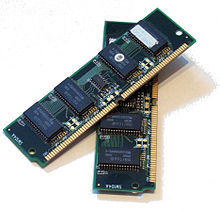
\includegraphics[width=0.45\textwidth]{figures/image/DRAM.jpg}
\cite{sumber : https://en.wikipedia.org/wiki/Dynamic_random-access_memory}
\caption{DRAM}
\label{labelgambar1}
\end{figure}

\item Sychronous Dynamic RAM disingkat SDRAM merupakan kelanjutan dari DRAM tetapi memiliki kecepatan yang lebih tinggi daripada DRAM dan telah disinkronisasi oleh clock sistem. DRAM ini cocok digunakan untuk sistem dengan bus yang memiliki kecepatan sampai 100 MHz.
\begin{figure}[htbp]
\centering
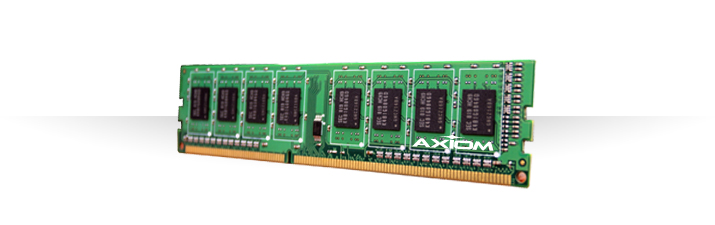
\includegraphics[width=0.45\textwidth]{figures/image/sdram.jpg}
\cite{sumber : http://axiommemory.com/categories/memory/Value-SDRAM.aspx}
\caption{SDRAM}
\label{labelgambar2}
\end{figure}

\item Dual In-line Memory Module disingkatan DIMM dari  berkapasitas 168 pin, kedua belah modul memori ini aktif, setiap permukaan adalah 84 pin. Berbeda dengan SIMM yang berfungsi hanya pada sebelah modul saja. Mensuport 64 bit penghantaran data. SDRAM
(Synchronous DRAM) menggunakan DIMM dan merupakan penganti dari DRAM, FPM (fast Page Memory) dan EDO. SDRAM memiliki fungsi untuk mengatur (synchronizes) memori supaya setara dengan CPU clock supaya pemindahan data yang dilakukan dapat dilakukan secara cepat. Terdapat dalam dua kecepatan yaitu 100MHz (PC100) dan 133MHz (PC133). DIMM 168 PIN. DIMM merupakan jenis RAM yang populer dan paling banyak terdapat di pasaran.
\begin{figure}[htbp]
\centering
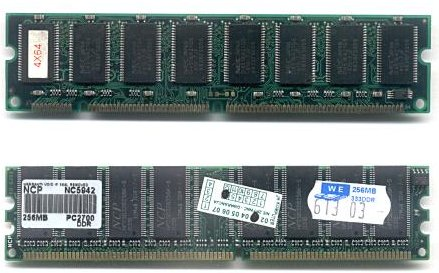
\includegraphics[width=0.45\textwidth]{figures/image/dimm.jpg}
\cite{sumber : https://en.wikipedia.org/wiki/DIMM}
\caption{DIMM}
\label{labelgambar3}
\end{figure}

\item Cache merupakan memori yang berkapasitas terbatas, namun memori ini memiliki kecepatan  yang tinggi dan lebih mahal dibandingkan memory utama. Cache ini terletak di antara register pemroses dan memori utama, dan memiliki fungsi agar pemroses tidak langsung mengacu kepada memori utama tetapi langsung di cache memory yang kecepatan aksesnya lebih tinggi, metode ini akan meningkatkan kinerja sistem. Cache memori merupakan salah satu tipe RAM tercepat yang pernah ada, dan digunakan oleh CPU, hard drive, dan beberapa pernah lainnya.

\item Magnetik Disk merupakan sebuah piringan bundar yang terbuat dari bahan tertentu seperti, logam atau plastik dengan permukaan dilapisi bahan - bahan yang dapat di magnetisasi. Mekanisme baca atau tulis menggunakan head atau kepala baca atau tulis yang dimana merupakan sebuah kumparan pengkonduksi (conducting coil ). Tampilan luar head bersifat stasioner sedangkan piringan disk berputar sesuai kontrolnya. Disk memiliki dua metode layout data, yaitu  constant angular velocity dan multiple zoned recording. Disk diorganisasikan dalam bentuk berupa cincin – cincin
Konsentris yang disebut track. Tiap track pada disk dipisahkan oleh gap. Gap digunakan sebagai pencegah atau mengantisipasi kesalahan penulisan maupun pembacaan yang disebabkan melesetnya head atau karena interferensi medan magnet. Sejumlah bit yang sama akan menempati track - track yang tersedia. Semakin dalam maka kerapatan dari disk akan bertambah besar. Biasanya data yang dikirim ke memori dalam bentuk blok - blok dan umumnya blok - blok tersebut lebih kecil kapasitasnya dari pada track. Blok - blok data yang disimpan dalam disk yang berukuran blok, yang disebut sektor. Sehingga track biasanya terisi beberapa sektor, umumnya 10 hingga 100 sektor tiap tracknya. Cara mekanisme pembacaan maupun penulisan pada disk dengan Head harus bisa mengidentifikasi titik awal atau posisi - posisi sektor maupun track. Caranya data yang disimpan akan diberi header data tambahan yang menginformasikan letak sektor dan track suatu data. Tipe memori Teknologi Ukuran Waktu akses Cache Memory semikonduktor RAM 128-512 KB 10 ns. Memori Utama semikonduktor RAM 4-128 MB 50 ns. Disk magnetik Hard Disk Gigabyte 10 ms, 10MB/det. Disk Optik CD-ROM Gigabyte 300ms, 600KB/det Pita magnetik Tape 100 MB De.
\begin{figure}[htbp]
\centering
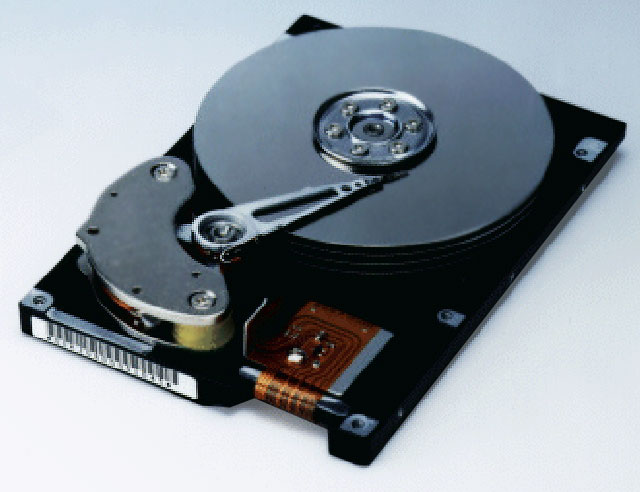
\includegraphics[width=0.45\textwidth]{figures/image/magnetic_disk.jpg}
\cite{sumber : http://museum.ipsj.or.jp/en/computer/device/magnetic_disk/0071.html}
\caption{Magnetc Disk}
\label{labelgambar3}
\end{figure}
\end{enumerate}


\section{Volatile non Volatile}
Volatile memory merupakan memory yang datanya dapat ditulis serta dihapus, tetapi akan hilang saat kehilangan power (kondisi off) serta membutuhkan suatu daya dalam mempertahankan memory. Contoh dari memory volatile yaitu RAM. RAM adalah memory utama PC yg bertugas untuk menerima sebuah informasi kemudian menyimpannya. kegunaannya sebgai penyimpanan sementara. 


Non-volatile memory merupakan memory yang datanya dapat ditulis serta dihapus, tetapi data akan tetap ada walaupun dalam kondisi off serta tidak membutuhkan suatu daya. Contoh dari memory Non volatile yaitu ROM. ROM adalah memory pada PC untuk menyimpan firmware. ROM bersifat permanen, artinya jika aliran listrik mati data yg tersimpan tidak akan terhapus


\section{Kecepatan Media Penyimpanan}
Perintah navigasi direktori